\documentclass[12pt]{beamer}
\usetheme{Madrid}
\usepackage[utf8]{inputenc}
\usepackage{amsmath}
\usepackage{amsfonts}
\usepackage{amssymb}
\usepackage{graphicx}
\usepackage{caption}
\usepackage{subcaption}
\setcounter{tocdepth}{4}
\setcounter{secnumdepth}{4}
\title{Convolutional Neural Networks}
%\setbeamercovered{transparent} 
%\setbeamertemplate{navigation symbols}{} 
%\logo{} 
%\institute{} 
%\date{} 
%\subject{} 

\author{
\linebreak
Julius Taylor \\ \texttt{0000000} \\ \href{mailto:stud3@email.com}{stud3@email.com}
 \and   
 \linebreak
Shawn Cala \\ \texttt{4921431} \\ \href{mailto:shawn.cala@gmail.com}{shawn.cala@gmail.com}
}

\begin{document}

\begin{frame}
\titlepage
\end{frame}
\frame{\frametitle{Table of Contents}\tableofcontents} 
%\begin{frame}
%\tableofcontents
%\end{frame}
\section{Background}
\subsection{Neural Networks}
\begin{frame}{Neural Networks}

Primary motivation: Neural Networks mathematically simulate biological functionalities of the human brain
\begin{figure}
\begin{subfigure}{.5\textwidth}
  \centering
  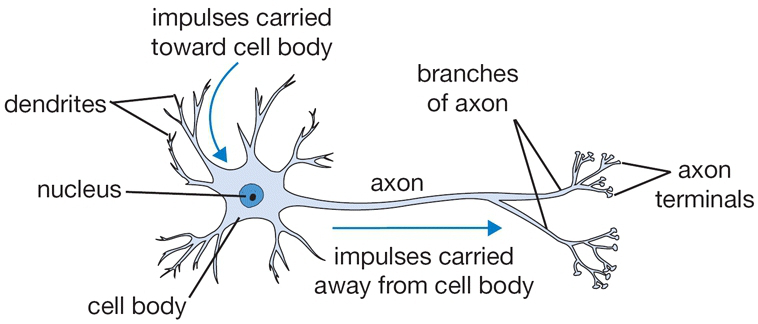
\includegraphics[width=\linewidth,height=0.35\textheight]{images/neuron.png}
  \caption{biological model}
  \label{fig:sub1}
\end{subfigure}%
\begin{subfigure}{.5\textwidth}
  \centering
  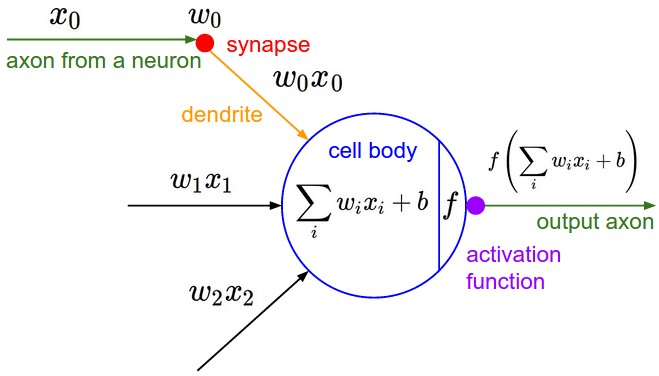
\includegraphics[width=\linewidth,height=0.35\textheight]{images/neuron_model.jpeg}
  \caption{mathematical representation}
  \label{fig:sub2}
\end{subfigure}
\caption{neuronal model and computational abstraction}
\label{fig:abstract}
\end{figure}

\end{frame}
\subsection{Structure}
\begin{frame}{Structure}
Neural Networks generally contain:
  \begin{itemize}
     \item an n-dimensional input 
     \item one or many layers of interconnected neurons
     \item an output-layer
  \end{itemize}
\begin{figure}
\centering
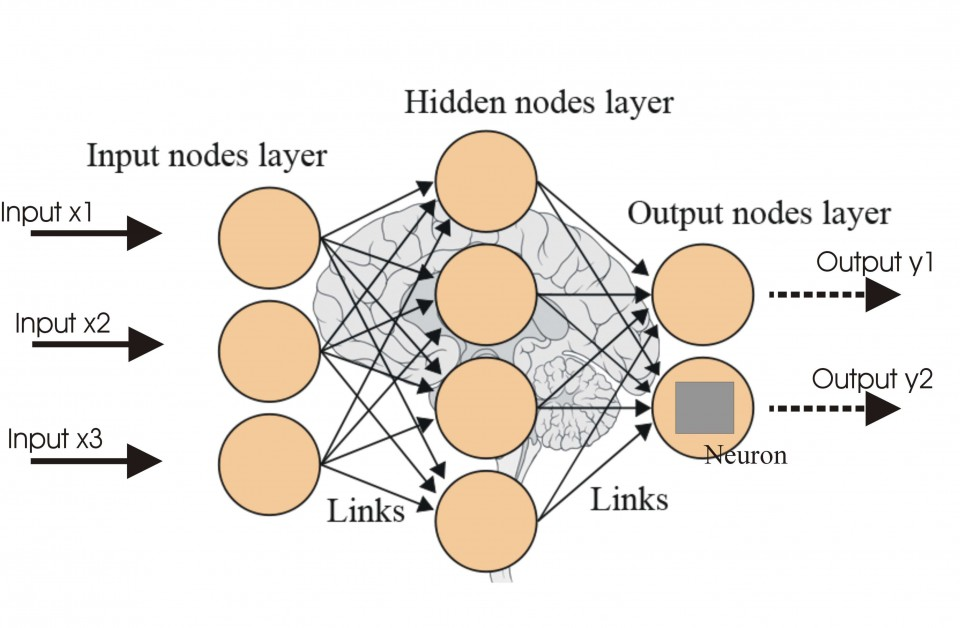
\includegraphics[width=0.5\linewidth]{images/principle.jpg}
\caption{Basic concept of a Neural Network}
\label{fig:principle}

\end{figure}

\end{frame}
\section{Convolutional Neural Networks}
\subsection{Concept}
\begin{frame}{Concept}
Convolutional Neural Networks (CNNs) are a subtype of Neural Networks:
  \begin{itemize}
     \item all neurons in a layer are identical 
     \item layers are interconnected through a kernel function
     \item different types of layers are used %(input, convolutional layer, RELU/tanh, maxpool,output
  \end{itemize}
\end{frame}
\begin{frame}{Background and Motivation - Convolutional Neural Networks}
\begin{figure}
\centering
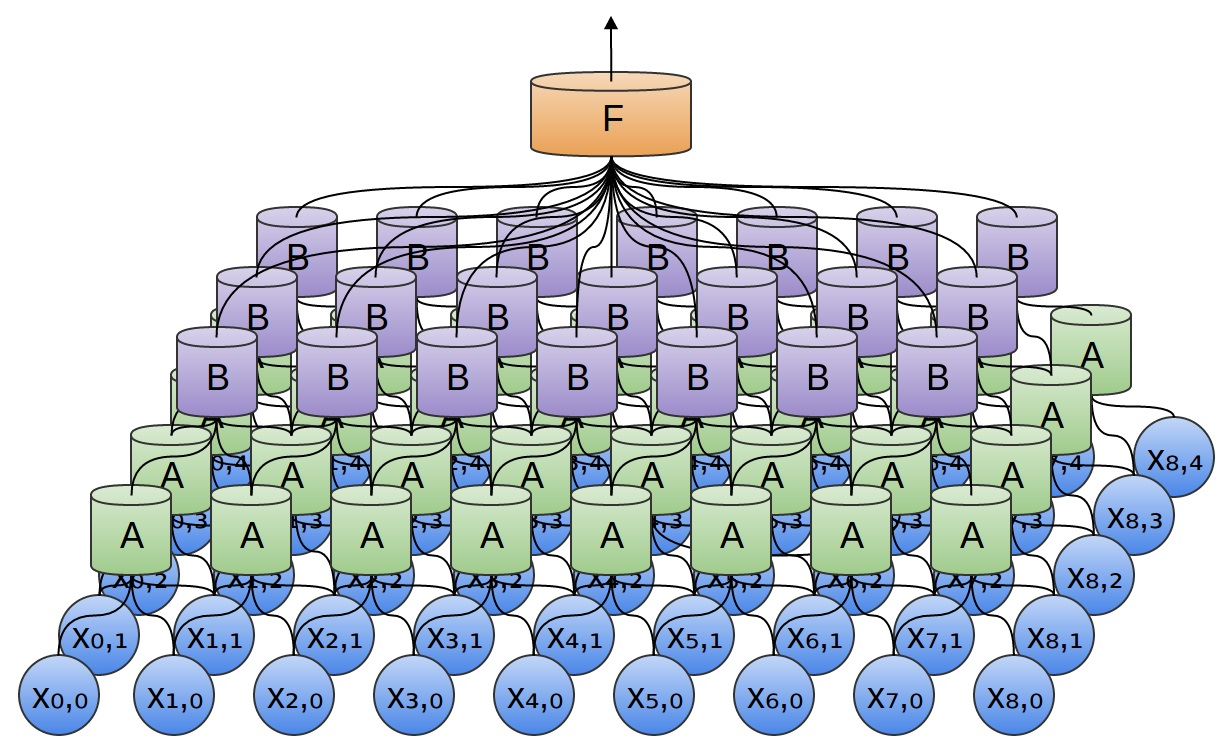
\includegraphics[width = 0.4\linewidth]{images/convexample.jpg}
\caption{2-dimensional CNN}
\label{fig:principle}
\end{figure}
\begin{enumerate}
\item Using identical copies of the same neuron allows for complex models with few parameters
\item Convolutional layers are not fully connected; each neurons is locally connected with a subsection of the previous layer.

This is represented mathematically through a kernel function.
\end{enumerate}
\end{frame}
\subsection{Kernel function}

\begin{frame}{Kernel function}
Kernel functions are an important component in many Neural Networks.
 \begin{figure}
\centering
e\includegraphics[width = 0.4\linewidth]{images/kernelfunction.png}
\caption{Forward propagation in a complex neural network}
todo: besseres Bild, vll gif mit kernelfunktion



\label{fig:propagation}
\end{figure}


\end{frame}

\subsection{Application}
\begin{frame}{Application}
Visual Object Recognition
\begin{figure}
\centering
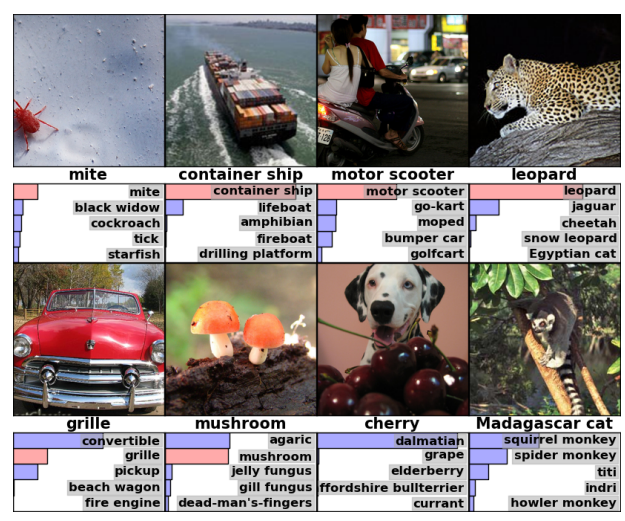
\includegraphics[width = 0.4\linewidth]{images/KSH-results.png}
\caption{ImageNet Classification with Deep Convolutional
Neural Networks}
\label{fig:principle}
\end{figure}
ImageNet by Krizhevsky et al (2012) classified 1.2 million
high-resolution images in the ImageNet LSVRC-2010 into 1000 different classes.
It achieves error rates of 37.5\% for the top result and 17.0\% for the top-5 results


%The neural network, which has 60 million parameters and 650,000 neurons, consists
%of five convolutional layers, some of which are followed by max-pooling layers,
%and three fully-connected layers with a final 1000-way softmax

\end{frame}

\begin{frame}{Application}
Text Classification
\begin{figure}
\centering
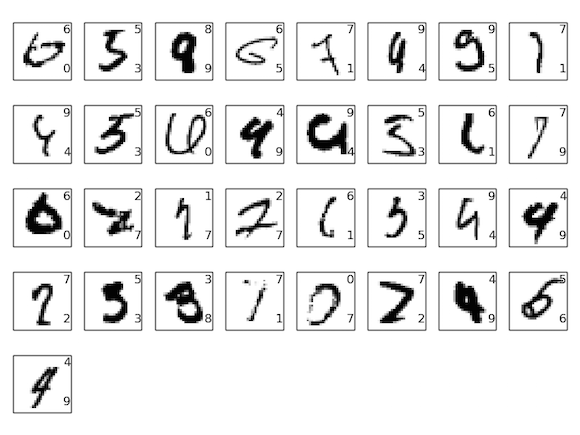
\includegraphics[width = 0.4\linewidth]{images/mnist.png}
\caption{Excerpt of mnist}
\label{fig:principle}
\end{figure}
fehlt: etwas Erklärung hierzu
\end{frame}








\section{Components}
\begin{frame}{Components}
hier Bild eines CNNs unseres Typs mit Komponenten


\begin{enumerate}
\item Neuron
\item Kernel-Function
\item Sigmoid function
\item softmax
\end{enumerate}

\end{frame}
\subsection{Activation function}
\begin{frame}{Activation Function}
Typically, an activation function is used  to add nonlinearity to the network
\begin{figure}
\centering
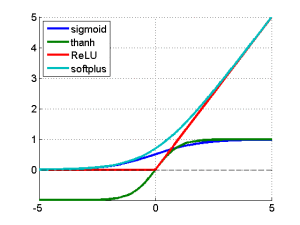
\includegraphics[width = 0.4\linewidth]{images/activation_functions.png}
\caption{Different activation functions}
\label{fig:principle}
\end{figure}
Activation functions must be non linear and differentiable. \newline
The employed network uses Sigmoid:

$\sigma(x) = \frac{1}{(1+e^(-x))}$



\end{frame}


\begin{frame}{Components - Neuron in fully connected layer}

\begin{figure}
\centering
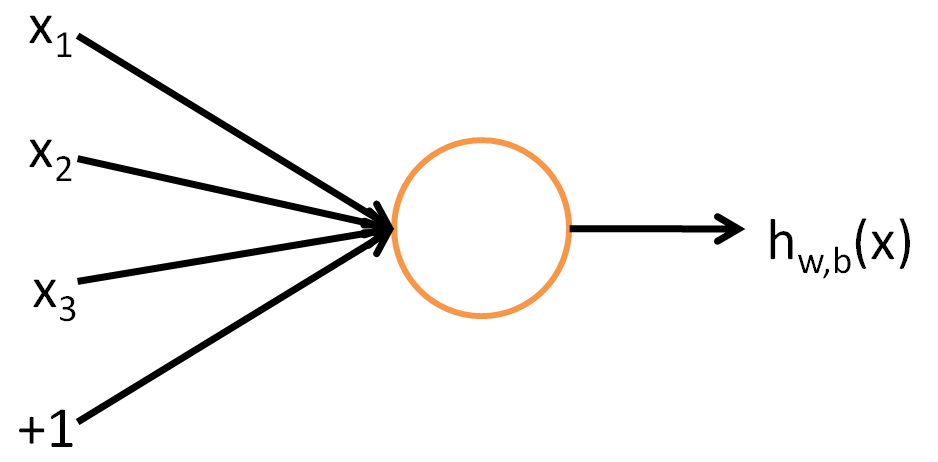
\includegraphics[width = 0.4\linewidth]{images/SingleNeuron.png}
\caption{Single neuron of a fully connected layer}
\label{fig:principle}
\end{figure}
Input: connected neurons from the previous layer \newline
Output: $f (\sum_{i}{w_i x_i})$

with \newline
$w_i$: 
\end{frame}




\begin{frame}{Components - Neuron in convolutional layer}
To understand the concept behind Convolution we first demonstrate it in an example:
\begin{figure}
\centering
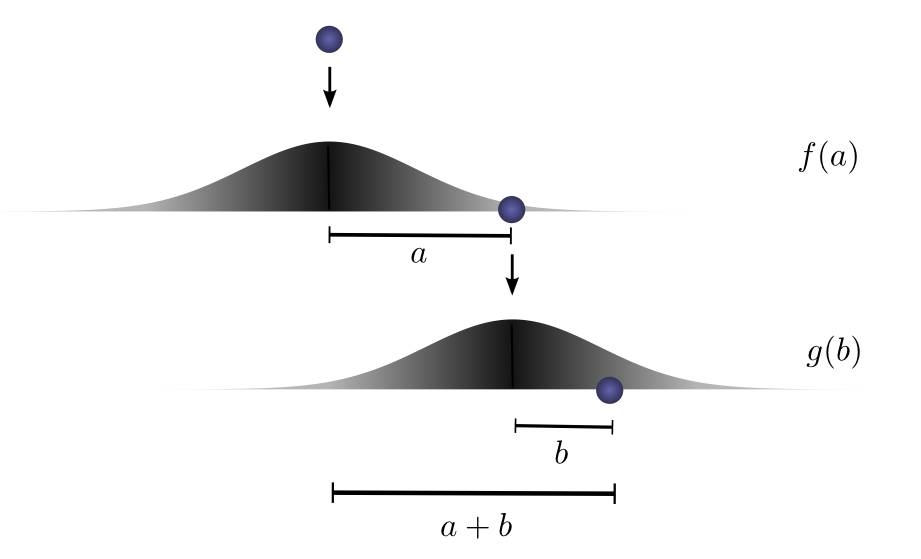
\includegraphics[width = 0.4\linewidth]{images/convprob.png}
\caption{Probability distribution of ball thrown twice}
\label{fig:principle}
\end{figure}
We want to calculate the likelihood of the ball traveling a distance $c$ after being thrown twice in a row. \newline


\end{frame}
\begin{frame}{Layers - Input}
\huge
Input layer
\newline
\normalsize
The input layer consists of an n-dimensional matrix, which contain the information to be processed

\begin{itemize}
\item Our example uses a 2-dimensional input which represents the pixels of the images
\item asd
\end{itemize}



\end{frame}


\begin{frame}
Input: \newline
$a, b$: length of first and second throw
$f(a), g(b)$: probability distribution of the balls location
If we want $c = a + b$ the probability of this event is $f(a) \cdot g(b)$

Since only the actual outcome is relevant to us, the actual values of $a$ and $b$ can be varied.

The total likelihood of the ball landing at $c$ can also be summed over all probability distributions where $a+b=c$:

$f*g(c) = \sum_{a+b=c} {f(a) \cdot g(a)} $

The result of this sum is a convolution between a and b
\end{frame}

\begin{frame}

\begin{figure}
\centering
Image processing with a kernel function can also be described as a convolution:
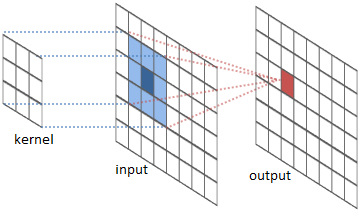
\includegraphics[width = 0.4\linewidth]{images/Kernelfunction.png}
\caption{Convolution between an input image and a kernel function}
\label{fig:principle}
\end{figure}

$out = \sum_{a} \sum_{b} w_{ab} \cdot x $



\end{frame}



\subsection{Backpropagation}
\begin{frame}{Backpropagation}

Backpropagation is the key algorithm which makes training Neural Networks feasible by greatly increasing the efficiency of learning algorithms.

To understand Backpropagation we first introduce the concept of forward propagation:

\end{frame}


\begin{frame}{Forward propagation}
Forward propagation is  the process of computing the output of a network for a given input



\begin{figure}
\centering
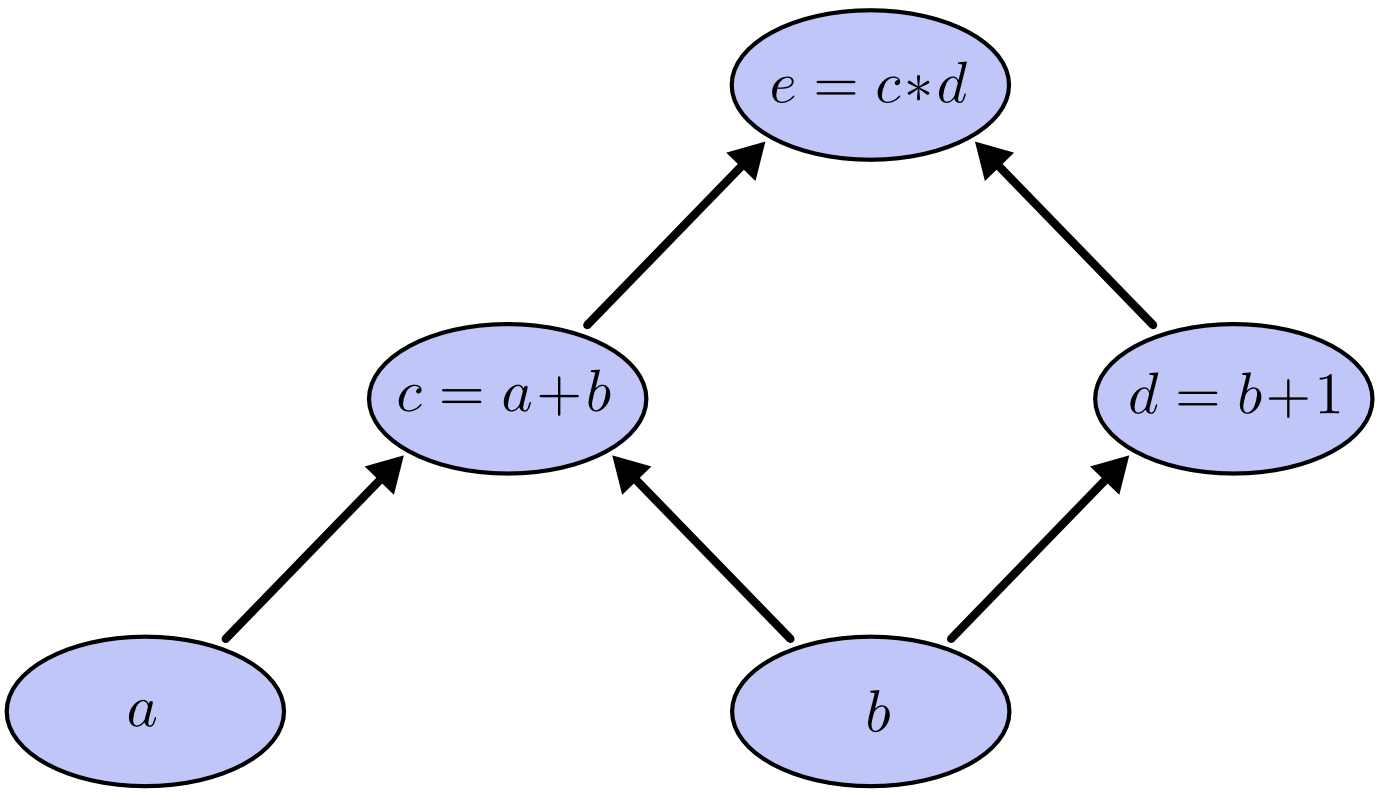
\includegraphics[width = 0.4\linewidth]{images/backprop1.png}
\caption{Computational graph of $e = (a+b)\cdot (b+1)$}

\label{fig:propagation}
\end{figure}
\end{frame}

\begin{frame}{Forward propagation}

We now arbitrarily set $a = 2$ and $b = 1$ for our example:

\begin{figure}
\centering
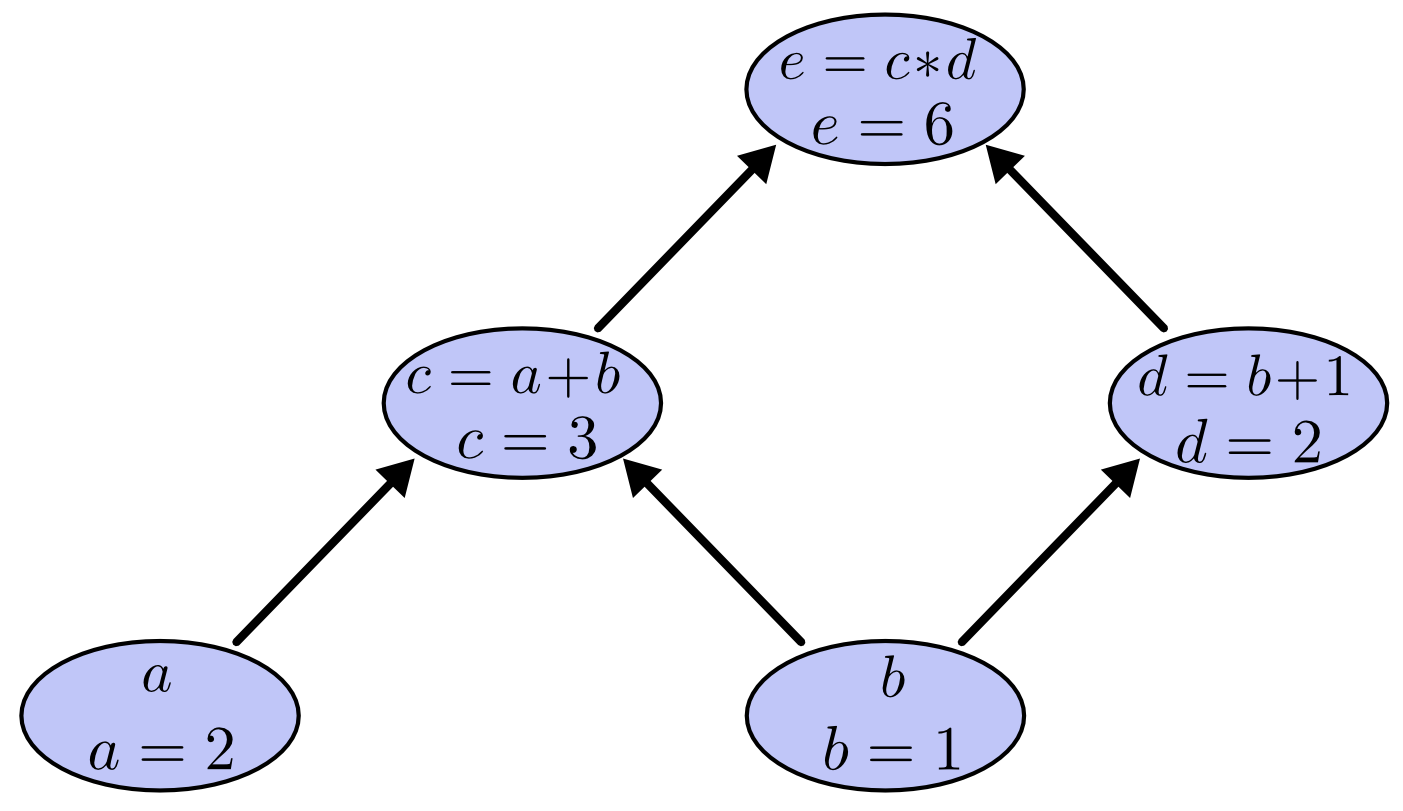
\includegraphics[width = 0.4\linewidth]{images/backprop2.png}
\caption{Computational graph of $e = (a+b)\cdot (b+1)$}

\label{fig:propagation}
\end{figure}
\end{frame}
\begin{frame}{Forward propagation}
If we want to train our network weights we must know how the output of the CNN is influenced by its layer weights.

In our example us would interest is how the result $e$ is influenced by $a$ and $b$
This is achieved by finding the respective partial derivatives
\begin{figure}
\centering
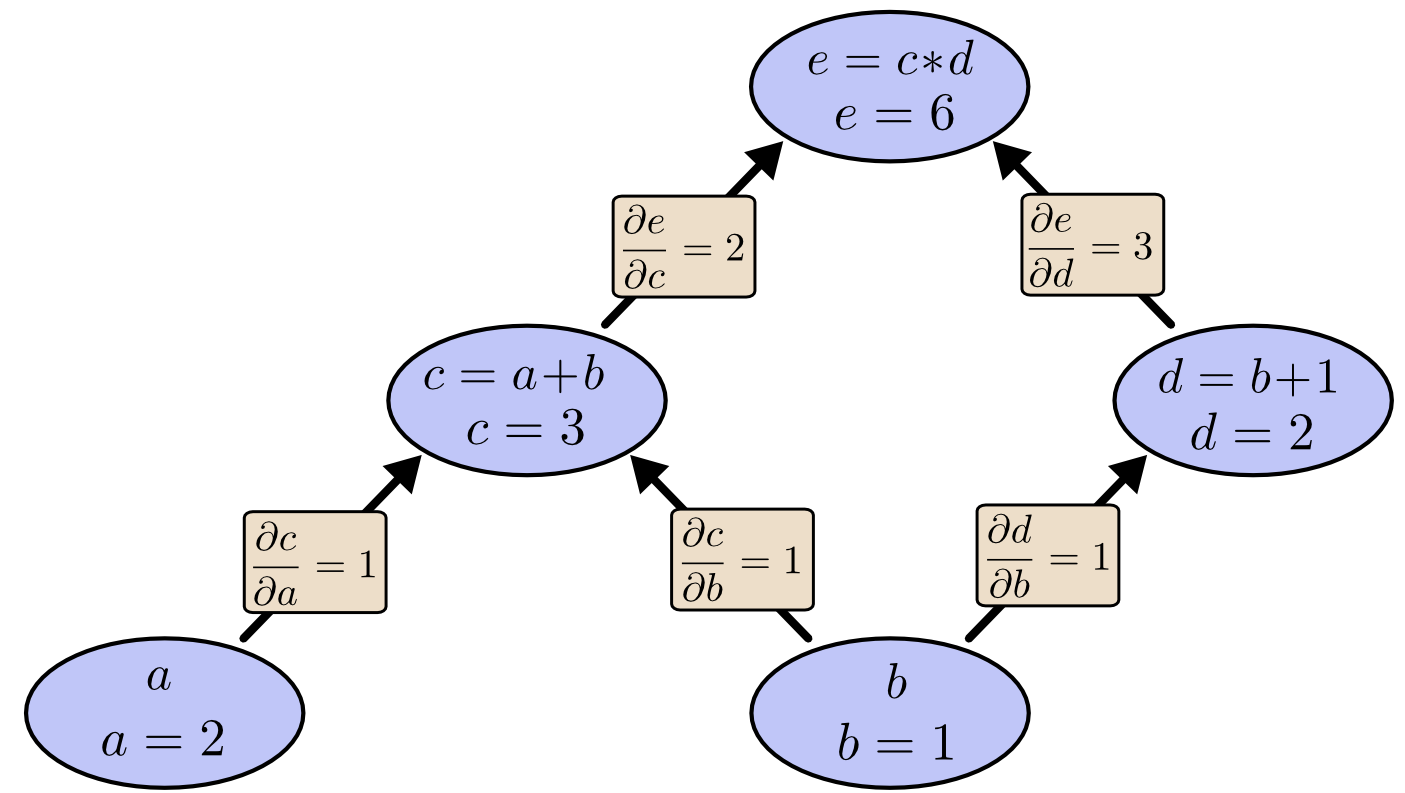
\includegraphics[width = 0.4\linewidth]{images/backprop3.png}
\caption{Partial derivatives}

\label{fig:propagation}
\end{figure}
$c$ is only indirectly influenced by $a$ and $b$. To derive the exact influence, the chain rule can be applied:
$\frac{\partial{e}}{\partial{a}} = \frac{\partial{e}}{\partial{c}} \cdot \frac{\partial{c}}{\partial{a}}$

$\frac{\partial{e}}{\partial{b}} = \frac{\partial{e}}{\partial{d}} \cdot \frac{\partial{e}}{\partial{c}} \cdot \frac{\partial{d}}{\partial{b}} \cdot \frac{\partial{c}}{\partial{b}}$

\end{frame}
\begin{frame}{Forward propagation}
In principle, this approach works for training a network
There are, however, obvious problems with exponential amounts of calculations if too many possible paths between input and output exist.
\begin{figure}
\centering
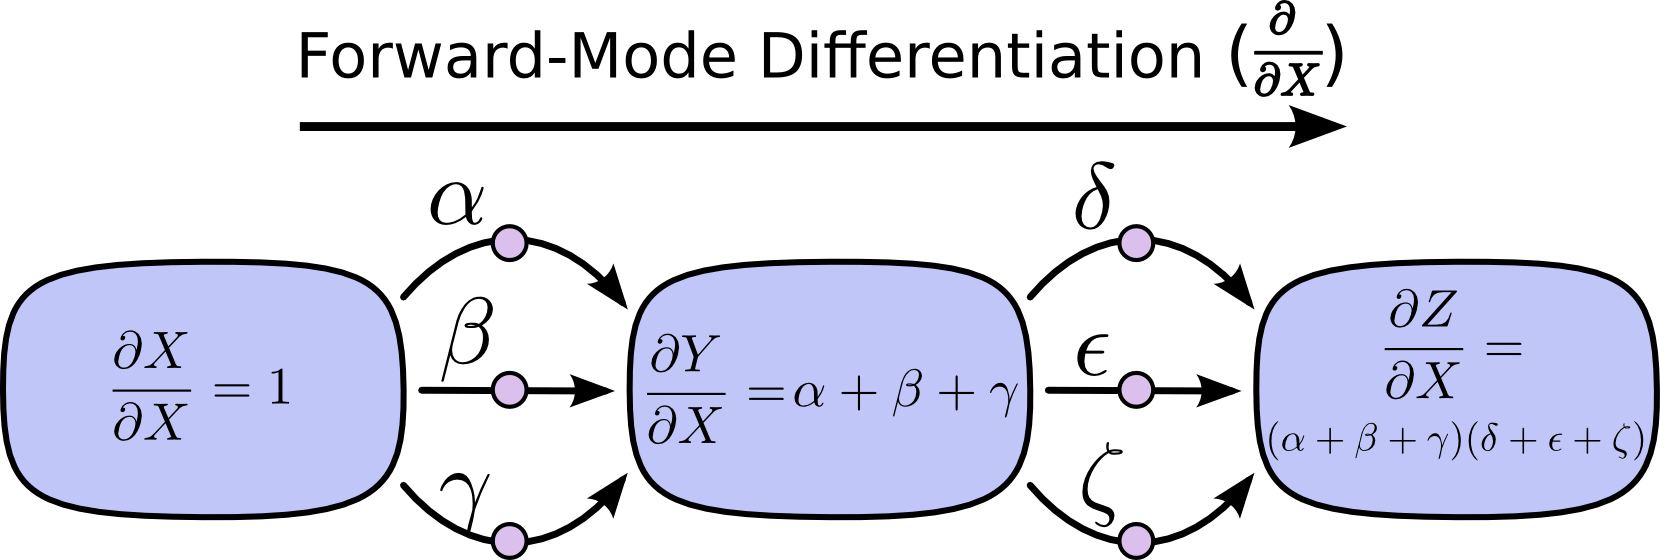
\includegraphics[width = 0.4\linewidth]{images/backprop5.png}
\label{fig:propagation5}
\end{figure}
\end{frame}

\begin{frame}{Backpropagation}
Instead of determining the influence of one input on the output we calculate how the output is influenced by the previous layer.

\begin{figure}
\centering
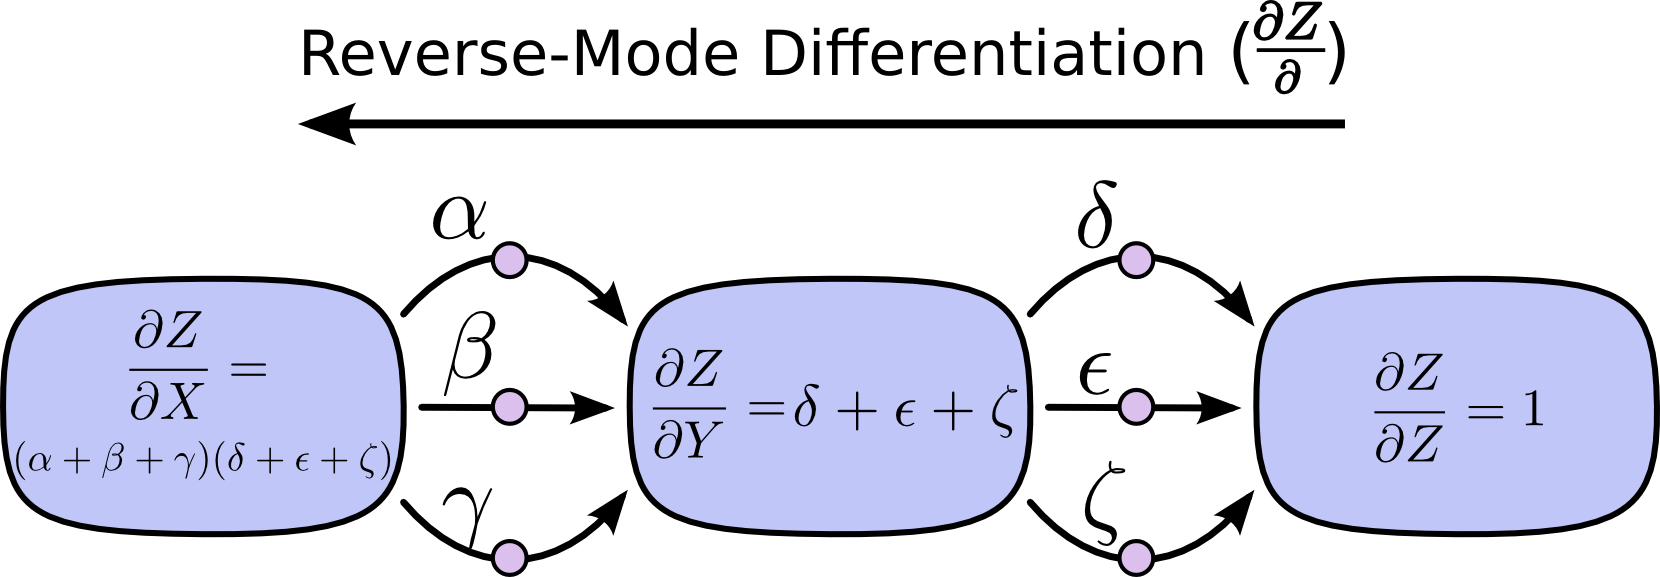
\includegraphics[width = 0.4\linewidth]{images/backprop6.png}
\label{fig:propagation5}
\end{figure}

\end{frame}

\begin{frame}{Backpropagation}
In our previous example executing a backward differentation immediately gives us the derivative of the output relative to every input.
 

\begin{figure}
\centering
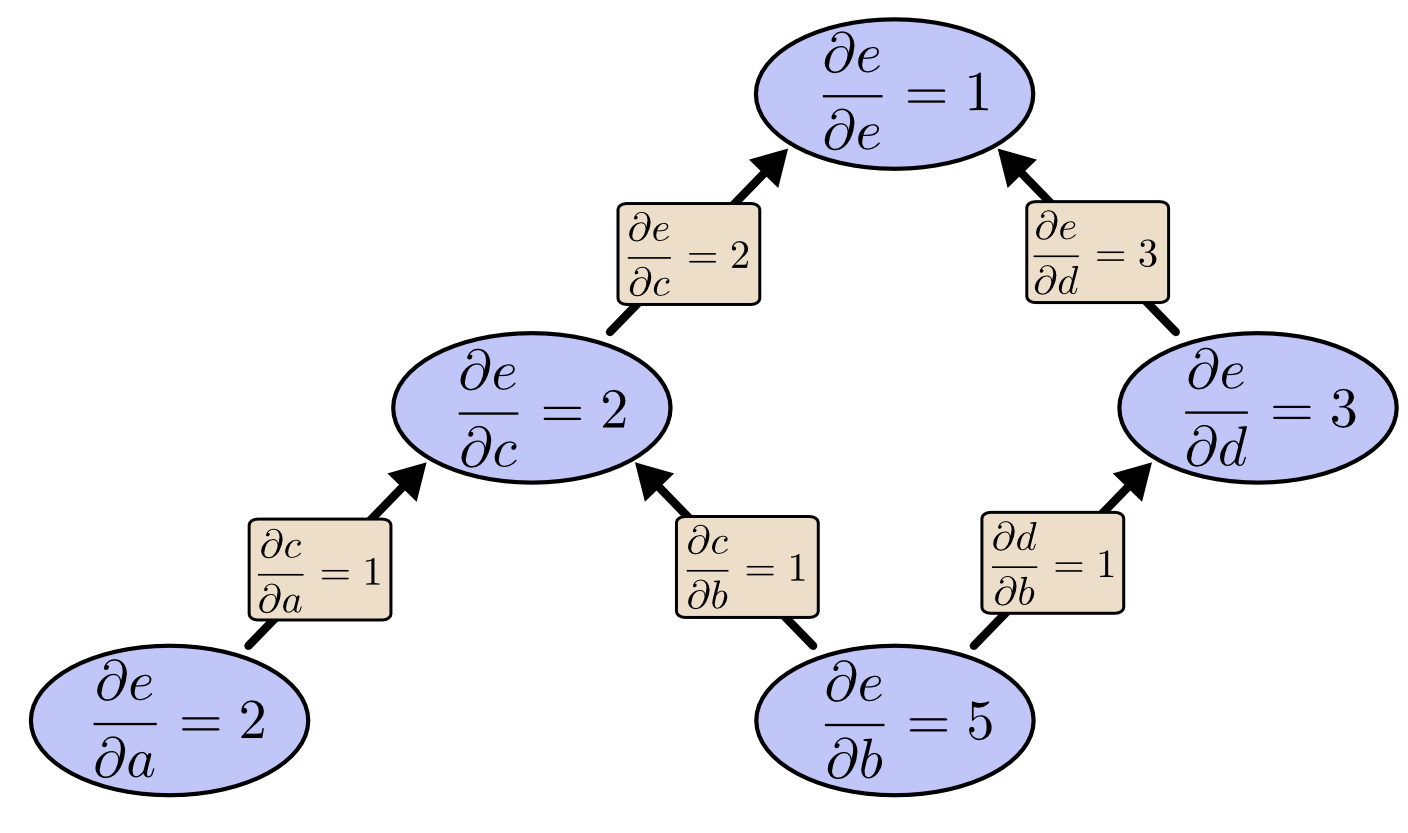
\includegraphics[width = 0.4\linewidth]{images/backprop7.png}
\label{fig:propagation5}
\end{figure}
=> massive speed in networks with many inputs/layers
\end{frame}

\begin{frame}{Backpropagation}
In our previous example executing a backward differentation immediately gives us the derivative of the output relative to every input.
 

\begin{figure}
\centering
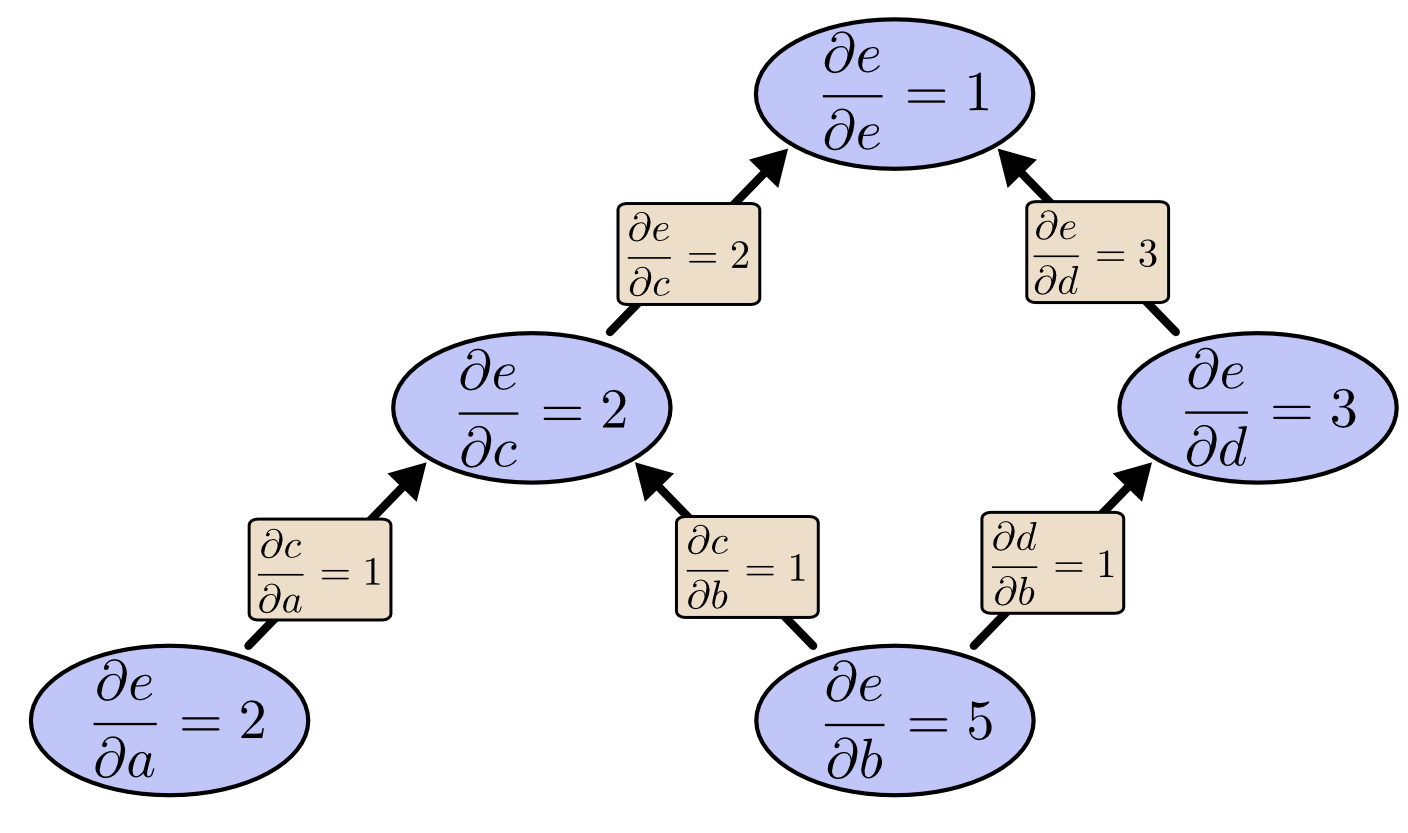
\includegraphics[width = 0.4\linewidth]{images/backprop7.png}
\label{fig:propagation5}
\end{figure}
=> massive speed in networks with many inputs/layers
\end{frame}


\begin{frame}{Backpropagation}
Lets  reiterate our network:

Convolution:                   $conv = x \cdot W_1 +b_1$ \newline
Convolutional layer output:    $out = tanh(conv)$\newline
Fully connected layer output:  $\hat{y} = out \cdot W_2 + b_2$\newline
Loss function:				   $L = - \sum_{N} y \cdot \ln{\hat{y}}$ \newline
\newline \newline
$\frac{\partial{L}}{\partial{W_2}} = \frac{\partial{L}}{\partial{\hat{y}}} \cdot \frac{\partial{\hat{y}}}{\partial{W_2}}$
\newline
$\frac{\partial{L}}{\partial{L}} = \sum_{N} y \cdot \frac{\partial{\ln{\hat{y}}}}{\partial{\hat{y}}} = \hat{y}-y$\newline
$\frac{\partial{\hat{y}}}{\partial{W_2}} = \frac{\partial{\hat{out \cdot W_2 +b_2 = out^T}}}{\partial{W_2}}$
$\frac{\partial{L}}{\partial{W_2}} = (\hat{y} - y) * out^T $
\end{frame}
\begin{frame}
$\frac{\partial{L}}{\partial{b_2}} = \frac{\partial{L}}{\partial{\hat{y}}} \cdot \frac{\partial{\hat{y}}}{\partial{b_2}}$\newline
$ = (\hat{y}-y) \cdot 1$\newline \newline
$\frac{\partial{L}}{\partial{W_1}} = \frac{\partial{L}}{\partial{\hat{y}}} \cdot \frac{\partial{\hat{y}}}{\partial{out}}\cdot \frac{\partial{out}}{\partial{conv}} \cdot \frac{\partial{conv}}{\partial{W_1}}$
\newline
$\frac{\partial{\hat{y}}}{\partial{out}} = \frac{\partial{\hat{out \cdot W_2 +b_2}}}{\partial{out}} =W_2$
$\frac{\partial{out}}{\partial{conv}} = \frac{\partial{ tanh(conv)}}{\partial{conv}} = 1 - \tanh^2{conv}$ 
$\frac{\partial{conv}}{\partial{W_1}} = x^T$

$\frac{\partial{L}}{\partial{W_1}} = x^T \cdot (1-tanh^2{conv} \cdot (y-\hat{y}) \cdot W_2 $



$\frac{\partial{L}}{\partial{b_1}} = \frac{\partial{L}}{\partial{\hat{y}}} \cdot \frac{\partial{\hat{y}}}{\partial{out}}\cdot \frac{\partial{out}}{\partial{conv}} \cdot \frac{\partial{conv}}{\partial{b_1}} = $

$ =  (1-tanh^2{conv} \cdot (y-\hat{y}) \cdot W_2 \cdot 1$




\end{frame}
\section{Problems}
\subsection{Overfitting}
\begin{frame} {Overfitting}

Overfitting occurs when the complexity of the model relative to the training size is too high.


The model begins memorizing the training data rather  than the underlying principle and easily loses its predictive power when the input is slightly altered.

Overfitting is prevented in a number of ways:

\begin{enumerate}

\item max-pooling layers
\item dropout layers
\item

\end{enumerate}

\end{frame}

\subsection{Underfitting}
\begin{frame}
\end{frame}
\section{Code}
\begin{frame}{Code}
\end{frame}


%todo: animal visual cortex
%\subsection{Layers}

%
%
%\begin{frame}{Layers - Convolution}
%The neurons of the Convolutional Layer is connected to the output of the previous layer through the kernel-function. 
%\end{frame}
%
%\begin{frame}{RELU/tanh layer}
%%The RELU layer (from rectified linear units) is a fully connected layer which implements the threshold function $y  = max(0,x)$. It adds non linearity to the network, which would otherwise be identical to a single layer perceptron. This makes the approximation of nonlinear functions possible. \newline Recent research has found a different activation function, the rectified linear function, often works better in practice for deep neural networks. This activation function is different from sigmoid and tanh http://ufldl.stanford.edu/tutorial/supervised/MultiLayerNeuralNetworks/
%
%because it is not bounded or continuously differentiable. The rectified linear activation function is given by,
%f(z)=max(0,x).
%
%To make backpropagation easier we used a differentiable function similar to RELU: $y = ln(1+e^x)$
%\end{frame}
%
%\begin{frame}{Max-Pooling layer}
%The Max-Pooling layer partitions the image, returns the maximum value of each partition   and returns a compressed version of the input. This is done to a) reduce overfitting and b) downsampling the input
%
%
%\end{frame}
%\begin{frame}{Dropout Layer}
%The dropout layer is a fully connected layer. It reduces overfitting and downsamples the input by randomly dropping neurons and their connections during training. 
%
%\end{frame}
%\begin{frame}{Dense layer}
%The dense layer is identical to a normal neural network layer in that it is fully interconnected with every neuron of the previous layer.
%\linebreak
%image here
%\end{frame}
%
%\begin{frame}{Output layer}
%The output layer is fully connected and unambigously assigns each neuron of the output to one of the expected results.
%\linebreak
%image here
%\end{frame}



\begin{thebibliography}{9}
\small
\bibitem{lamport94}
  Leslie Lamport,
  \emph{\LaTeX: a document preparation system},
  Addison Wesley, Massachusetts,
  2nd edition,
  1994.
@misc{bworld,
  author = {Christian Perone},
  title = {{Deep learning – Convolutional neural networks and feature extraction with Python}},
  howpublished = "\url{http://blog.christianperone.com/2015/08/convolutional-neural-networks-and-feature-extraction-with-python/}",
  year = {2015}, 
  note = "[Online; accessed 21.01.2017]"
}
%figures 1 and 2 from http://cs231n.github.io/neural-networks-1/#bio
%figure 3 http://futurehumanevolution.com/artificial-intelligence-future-human-evolution/artificial-neural-networks
% figure 4 http://colah.github.io/posts/2014-07-Conv-Nets-Modular/
% https://bfeba431-a-62cb3a1a-s-sites.googlegroups.com/site/deeplearningcvpr2014/ranzato_cvpr2014_DLtutorial.pdf?attachauth=ANoY7cpoT6OKao2g3iqQB4JqrLBF4e9GfZ06wOsnqfD_Dy5aob09rA3XzGPQSysUphYafHjkncEfoJPPyab19s4v8tfQS65Xk57NWieQOFC1zrYR2O_0gUN1Bsb64TS6kucrQP2prHjwwO4-Bc_9IRzGfWtlSMUGL_SxZnW_uSJHNbCzTQSfeZicjRxOCsBCNcA-4ifO2z8HaCqegyP8LQQGlp9gA7bPiIva1wxa69xKa7PB0iipEVWW180McZkDbBjefD0Thr13&attredirects=0
%figure forward propagation http://briandolhansky.com/blog/2013/9/27/artificial-neural-networks-backpropagation-part-4
% back propagation: http://neuralnetworksanddeeplearning.com/chap2.html
% Kernel function + KSH results http://colah.github.io/posts/2014-07-Understanding-Convolutions/
% mnist image: http://neuralnetworksanddeeplearning.com/chap6.html
% single neuron http://ufldl.stanford.edu/tutorial/supervised/MultiLayerNeuralNetworks/
% activation function image: https://imiloainf.wordpress.com/2013/11/06/rectifier-nonlinearities/
% two balls image: http://colah.github.io/posts/2014-07-Understanding-Convolutions/
% images on backprop https://colah.github.io/posts/2015-08-Backprop/
http://cs231n.github.io/convolutional-networks/
http://colah.github.io/posts/2014-07-Conv-Nets-Modular/
http://www.cs.toronto.edu/~fritz/absps/imagenet.pdf
\end{thebibliography}
\end{document}